\documentclass[twoside]{book}

% Packages required by doxygen
\usepackage{fixltx2e}
\usepackage{calc}
\usepackage{doxygen}
\usepackage{graphicx}
\usepackage[utf8]{inputenc}
\usepackage{makeidx}
\usepackage{multicol}
\usepackage{multirow}
\PassOptionsToPackage{warn}{textcomp}
\usepackage{textcomp}
\usepackage[nointegrals]{wasysym}
\usepackage[table]{xcolor}

% Font selection
\usepackage[T1]{fontenc}
\usepackage{mathptmx}
\usepackage[scaled=.90]{helvet}
\usepackage{courier}
\usepackage{amssymb}
\usepackage{sectsty}
\renewcommand{\familydefault}{\sfdefault}
\allsectionsfont{%
  \fontseries{bc}\selectfont%
  \color{darkgray}%
}
\renewcommand{\DoxyLabelFont}{%
  \fontseries{bc}\selectfont%
  \color{darkgray}%
}
\newcommand{\+}{\discretionary{\mbox{\scriptsize$\hookleftarrow$}}{}{}}

% Page & text layout
\usepackage{geometry}
\geometry{%
  a4paper,%
  top=2.5cm,%
  bottom=2.5cm,%
  left=2.5cm,%
  right=2.5cm%
}
\tolerance=750
\hfuzz=15pt
\hbadness=750
\setlength{\emergencystretch}{15pt}
\setlength{\parindent}{0cm}
\setlength{\parskip}{0.2cm}
\makeatletter
\renewcommand{\paragraph}{%
  \@startsection{paragraph}{4}{0ex}{-1.0ex}{1.0ex}{%
    \normalfont\normalsize\bfseries\SS@parafont%
  }%
}
\renewcommand{\subparagraph}{%
  \@startsection{subparagraph}{5}{0ex}{-1.0ex}{1.0ex}{%
    \normalfont\normalsize\bfseries\SS@subparafont%
  }%
}
\makeatother

% Headers & footers
\usepackage{fancyhdr}
\pagestyle{fancyplain}
\fancyhead[LE]{\fancyplain{}{\bfseries\thepage}}
\fancyhead[CE]{\fancyplain{}{}}
\fancyhead[RE]{\fancyplain{}{\bfseries\leftmark}}
\fancyhead[LO]{\fancyplain{}{\bfseries\rightmark}}
\fancyhead[CO]{\fancyplain{}{}}
\fancyhead[RO]{\fancyplain{}{\bfseries\thepage}}
\fancyfoot[LE]{\fancyplain{}{}}
\fancyfoot[CE]{\fancyplain{}{}}
\fancyfoot[RE]{\fancyplain{}{\bfseries\scriptsize Generated on Sat Nov 22 2014 14\+:42\+:26 for C\+A\+L\+C\+U\+L\+A\+T\+O\+R by Doxygen }}
\fancyfoot[LO]{\fancyplain{}{\bfseries\scriptsize Generated on Sat Nov 22 2014 14\+:42\+:26 for C\+A\+L\+C\+U\+L\+A\+T\+O\+R by Doxygen }}
\fancyfoot[CO]{\fancyplain{}{}}
\fancyfoot[RO]{\fancyplain{}{}}
\renewcommand{\footrulewidth}{0.4pt}
\renewcommand{\chaptermark}[1]{%
  \markboth{#1}{}%
}
\renewcommand{\sectionmark}[1]{%
  \markright{\thesection\ #1}%
}

% Indices & bibliography
\usepackage{natbib}
\usepackage[titles]{tocloft}
\setcounter{tocdepth}{3}
\setcounter{secnumdepth}{5}
\makeindex

% Hyperlinks (required, but should be loaded last)
\usepackage{ifpdf}
\ifpdf
  \usepackage[pdftex,pagebackref=true]{hyperref}
\else
  \usepackage[ps2pdf,pagebackref=true]{hyperref}
\fi
\hypersetup{%
  colorlinks=true,%
  linkcolor=blue,%
  citecolor=blue,%
  unicode%
}

% Custom commands
\newcommand{\clearemptydoublepage}{%
  \newpage{\pagestyle{empty}\cleardoublepage}%
}


%===== C O N T E N T S =====

\begin{document}

% Titlepage & ToC
\hypersetup{pageanchor=false,
             bookmarks=true,
             bookmarksnumbered=true,
             pdfencoding=unicode
            }
\pagenumbering{roman}
\begin{titlepage}
\vspace*{7cm}
\begin{center}%
{\Large C\+A\+L\+C\+U\+L\+A\+T\+O\+R }\\
\vspace*{1cm}
{\large Generated by Doxygen 1.8.8}\\
\vspace*{0.5cm}
{\small Sat Nov 22 2014 14:42:26}\\
\end{center}
\end{titlepage}
\clearemptydoublepage
\tableofcontents
\clearemptydoublepage
\pagenumbering{arabic}
\hypersetup{pageanchor=true}

%--- Begin generated contents ---
\chapter{Developing-\/\+Computer-\/\+Programming-\/\+Program-\/\+Elements-\/\+Structure}
\label{md__developing_programming__developing_computer_programming__r_e_a_d_m_e}
\hypertarget{md__developing_programming__developing_computer_programming__r_e_a_d_m_e}{}
Developing Computer Programming\+: Program Elements \& Structure, challenges, programs and documentation 
\chapter{File Index}
\section{File List}
Here is a list of all files with brief descriptions\+:\begin{DoxyCompactList}
<<<<<<< HEAD
\item\contentsline{section}{Developing\+Programming/\+Teacher\+Basics/\hyperlink{_teacher_basics_8c}{Teacher\+Basics.\+c} }{\pageref{_teacher_basics_8c}}{}
=======
\item\contentsline{section}{/\+Users/nishantjain/\+Desktop/\+Developing\+Programming/\+Teacehr\+Basics/\hyperlink{_teacher_basics_8c}{Teacher\+Basics.\+c} }{\pageref{_teacher_basics_8c}}{}
>>>>>>> master
\end{DoxyCompactList}

\chapter{File Documentation}
\hypertarget{_expression_calc_8c}{\section{Developing\+Programming/\+Developing\+Computer\+Programming/\+Expression\+Calc.c File Reference}
\label{_expression_calc_8c}\index{Developing\+Programming/\+Developing\+Computer\+Programming/\+Expression\+Calc.\+c@{Developing\+Programming/\+Developing\+Computer\+Programming/\+Expression\+Calc.\+c}}
}
{\ttfamily \#include $<$stdio.\+h$>$}\\*
{\ttfamily \#include $<$stdlib.\+h$>$}\\*
Include dependency graph for Expression\+Calc.\+c\+:\nopagebreak
\begin{figure}[H]
\begin{center}
\leavevmode
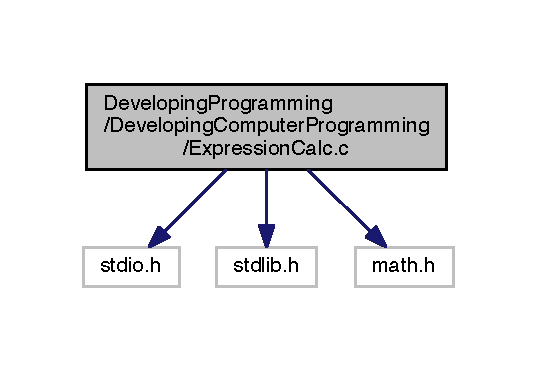
\includegraphics[width=252pt]{_expression_calc_8c__incl}
\end{center}
\end{figure}
\subsection*{Functions}
\begin{DoxyCompactItemize}
\item 
void \hyperlink{_expression_calc_8c_a79cd2ba7236d8017474e3340e169f888}{Extra} ()
\begin{DoxyCompactList}\small\item\em Function to use Extra features of the Calculator. \end{DoxyCompactList}\item 
void \hyperlink{_expression_calc_8c_a1f044085ede204d3d2ba2e4db44e7e5d}{Calc\+Fib} (int r)
\begin{DoxyCompactList}\small\item\em Function to print Fibonacci Series according to input of the range by the user. \end{DoxyCompactList}\item 
int \hyperlink{_expression_calc_8c_ae66f6b31b5ad750f1fe042a706a4e3d4}{main} ()
\end{DoxyCompactItemize}


\subsection{Function Documentation}
\hypertarget{_expression_calc_8c_a1f044085ede204d3d2ba2e4db44e7e5d}{\index{Expression\+Calc.\+c@{Expression\+Calc.\+c}!Calc\+Fib@{Calc\+Fib}}
\index{Calc\+Fib@{Calc\+Fib}!Expression\+Calc.\+c@{Expression\+Calc.\+c}}
\subsubsection[{Calc\+Fib}]{\setlength{\rightskip}{0pt plus 5cm}void Calc\+Fib (
\begin{DoxyParamCaption}
\item[{int}]{r}
\end{DoxyParamCaption}
)}}\label{_expression_calc_8c_a1f044085ede204d3d2ba2e4db44e7e5d}


Function to print Fibonacci Series according to input of the range by the user. 



Definition at line \hyperlink{_expression_calc_8c_source_l00109}{109} of file \hyperlink{_expression_calc_8c_source}{Expression\+Calc.\+c}.



Referenced by \hyperlink{_expression_calc_8c_source_l00096}{Extra()}.


\begin{DoxyCode}
00110 \{
00111   \textcolor{keywordtype}{int} j=0, k=1, res;
00112   printf(\textcolor{stringliteral}{"FIBONACCI SERIES: "});
00113   
00114   \textcolor{comment}{//printing first two values.}
00115   printf(\textcolor{stringliteral}{"%d %d"},j,k); 
00116 
00117     \textcolor{keywordflow}{for}(\textcolor{keywordtype}{int} i=2;i<r;i++)
00118     \{
00119       res=j+k;
00120       j=k;
00121       k=res; 
00122       printf(\textcolor{stringliteral}{" %d"},k);
00123     \}  
00124   printf(\textcolor{stringliteral}{"\(\backslash\)n"}); 
00125 \}
\end{DoxyCode}


Here is the caller graph for this function\+:\nopagebreak
\begin{figure}[H]
\begin{center}
\leavevmode
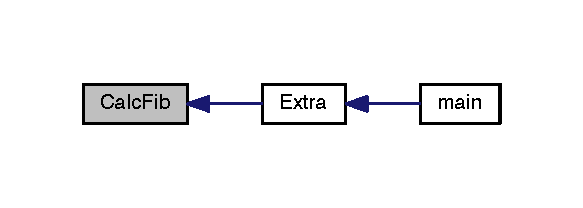
\includegraphics[width=280pt]{_expression_calc_8c_a1f044085ede204d3d2ba2e4db44e7e5d_icgraph}
\end{center}
\end{figure}


\hypertarget{_expression_calc_8c_a79cd2ba7236d8017474e3340e169f888}{\index{Expression\+Calc.\+c@{Expression\+Calc.\+c}!Extra@{Extra}}
\index{Extra@{Extra}!Expression\+Calc.\+c@{Expression\+Calc.\+c}}
\subsubsection[{Extra}]{\setlength{\rightskip}{0pt plus 5cm}void Extra (
\begin{DoxyParamCaption}
{}
\end{DoxyParamCaption}
)}}\label{_expression_calc_8c_a79cd2ba7236d8017474e3340e169f888}


Function to use Extra features of the Calculator. 



Definition at line \hyperlink{_expression_calc_8c_source_l00096}{96} of file \hyperlink{_expression_calc_8c_source}{Expression\+Calc.\+c}.



References \hyperlink{_expression_calc_8c_source_l00109}{Calc\+Fib()}.



Referenced by \hyperlink{_expression_calc_8c_source_l00008}{main()}.


\begin{DoxyCode}
00097 \{ 
00098   \textcolor{keywordtype}{int} ch,r;
00099   printf(\textcolor{stringliteral}{"\(\backslash\)nSelect from the following options: \(\backslash\)n1)Fibonacci Series \(\backslash\)n"});
00100   scanf(\textcolor{stringliteral}{" %d"},&ch);
00101   \textcolor{keywordflow}{switch}(ch)
00102   \{
00103     \textcolor{keywordflow}{case} 1: printf(\textcolor{stringliteral}{"Enter the range of Fibonacci series: \(\backslash\)n "}); scanf(\textcolor{stringliteral}{" %d"},&r); 
      \hyperlink{_expression_calc_8c_a1f044085ede204d3d2ba2e4db44e7e5d}{CalcFib}(r); \textcolor{keywordflow}{break};
00104   \}
00105 \}
\end{DoxyCode}


Here is the call graph for this function\+:\nopagebreak
\begin{figure}[H]
\begin{center}
\leavevmode
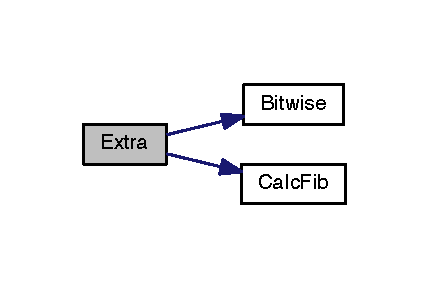
\includegraphics[width=206pt]{_expression_calc_8c_a79cd2ba7236d8017474e3340e169f888_cgraph}
\end{center}
\end{figure}




Here is the caller graph for this function\+:\nopagebreak
\begin{figure}[H]
\begin{center}
\leavevmode
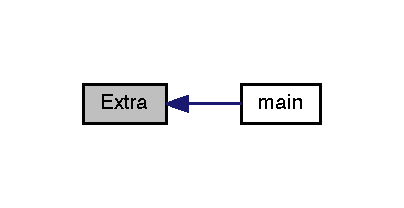
\includegraphics[width=194pt]{_expression_calc_8c_a79cd2ba7236d8017474e3340e169f888_icgraph}
\end{center}
\end{figure}


\hypertarget{_expression_calc_8c_ae66f6b31b5ad750f1fe042a706a4e3d4}{\index{Expression\+Calc.\+c@{Expression\+Calc.\+c}!main@{main}}
\index{main@{main}!Expression\+Calc.\+c@{Expression\+Calc.\+c}}
\subsubsection[{main}]{\setlength{\rightskip}{0pt plus 5cm}int main (
\begin{DoxyParamCaption}
{}
\end{DoxyParamCaption}
)}}\label{_expression_calc_8c_ae66f6b31b5ad750f1fe042a706a4e3d4}


Definition at line \hyperlink{_expression_calc_8c_source_l00008}{8} of file \hyperlink{_expression_calc_8c_source}{Expression\+Calc.\+c}.



References \hyperlink{_expression_calc_8c_source_l00096}{Extra()}.


\begin{DoxyCode}
00009 \{
00010   \textcolor{comment}{//Welcome Screen}
00011   printf(\textcolor{stringliteral}{"Welcome to Calculator. \(\backslash\)n"});                          
00012   \textcolor{keywordtype}{char} check;
00013   \textcolor{keywordtype}{int} r;
00014   \textcolor{keywordtype}{int} ch;
00015   \textcolor{keywordtype}{char} opt;
00016   \textcolor{keywordtype}{float} var1, var2;
00017   \textcolor{keywordtype}{float} res;
00018   FILE * Log;
00019   
00020   \textcolor{comment}{//Opening a new file for Logging info. Opening in reading and writing mode}
00021   Log = fopen (\textcolor{stringliteral}{"Log.txt"}, \textcolor{stringliteral}{"w+"});                            
00022       
00023     \textcolor{keywordflow}{do}
00024     \{                                                           
00025       printf(\textcolor{stringliteral}{"Please select an Arithmetic operation from the following: \(\backslash\)n"});           
00026       printf(\textcolor{stringliteral}{"1)Addition \(\backslash\)t 2)Subtraction \(\backslash\)t 3)Multiplication \(\backslash\)t 4)Division \(\backslash\)t 5)Extra Features \(\backslash\)n "});
00027       
00028       \textcolor{comment}{//Input of operation, A SPACE before %d makes scanf ignore whitespace}
00029       scanf(\textcolor{stringliteral}{" %d"}, &ch);                                            
00030       
00031       \textcolor{keywordflow}{if}(ch!=5)
00032       \{
00033         \textcolor{comment}{//Asking user if he wants to use saved previous result}
00034         printf(\textcolor{stringliteral}{"Do you want to use the previous result as one of the operands (Y/N)? \(\backslash\)n"});
00035         scanf(\textcolor{stringliteral}{" %c"}, &opt);                                                 
00036       
00037         printf(\textcolor{stringliteral}{"Enter any values for operand(s): \(\backslash\)n"});
00038         \textcolor{keywordflow}{if}(opt==\textcolor{charliteral}{'Y'} || opt==\textcolor{charliteral}{'y'})
00039           \{
00040             printf(\textcolor{stringliteral}{"Operand 1 is the previous result: "});
00041             rewind(Log);
00042             \textcolor{comment}{//Taking value from the LOG text file for variable 1}
00043             fscanf(Log, \textcolor{stringliteral}{" %f"}, &var1);                                  
00044             printf(\textcolor{stringliteral}{"%f \(\backslash\)n"}, var1);
00045           \}  
00046       
00047         \textcolor{keywordflow}{else} 
00048         \{
00049           printf(\textcolor{stringliteral}{"Operand 1: "}); 
00050           scanf(\textcolor{stringliteral}{"%f"}, &var1);                                       
00051         \}
00052         
00053         printf(\textcolor{stringliteral}{"Operand 2: "}); 
00054         \textcolor{comment}{/* An optional starting asterisk or space indicates }
00055 \textcolor{comment}{        *that the data is to be read from the stream but }
00056 \textcolor{comment}{        *ignored, i.e. it is not stored in the corresponding argument.  }
00057 \textcolor{comment}{        *Input of variable2 */}
00058         
00059         scanf(\textcolor{stringliteral}{" %f"}, &var2);
00060         
00061         \textcolor{comment}{//Switch case construct: Statements for different conditions }
00062         \textcolor{keywordflow}{switch}(ch)                                              
00063         \{
00064           \textcolor{keywordflow}{case} 1: res=var1+var2; \textcolor{keywordflow}{break};
00065           \textcolor{keywordflow}{case} 2: res=var1-var2; \textcolor{keywordflow}{break};
00066           \textcolor{keywordflow}{case} 3: res=var1*var2; \textcolor{keywordflow}{break};
00067           \textcolor{keywordflow}{case} 4: res=var1/var2; \textcolor{keywordflow}{break};
00068         \}
00069          
00070         \textcolor{comment}{//Displaying result from file}
00071         printf(\textcolor{stringliteral}{"\(\backslash\)nThe Result= %f \(\backslash\)n"}, res);                         
00072       
00073         rewind(Log);
00074         \textcolor{comment}{//Logging the result}
00075         fprintf(Log, \textcolor{stringliteral}{" %f"}, res);                               
00076       
00077       \}
00078       
00079       \textcolor{comment}{//Calling the CalcFib() function and passing range as parameter.}
00080       \textcolor{keywordflow}{else} \hyperlink{_expression_calc_8c_a79cd2ba7236d8017474e3340e169f888}{Extra}();                                     
00081       
00082       \textcolor{comment}{//Asking user to continue or exit}
00083       printf(\textcolor{stringliteral}{"Continue y/n?  "});                                
00084       scanf(\textcolor{stringliteral}{" %c"},&check);                                      
00085       
00086     \}\textcolor{keywordflow}{while}(check!=\textcolor{charliteral}{'n'});                 
00087    
00088     \textcolor{comment}{// Closing opened text file}
00089     fclose(Log);                                                    
00090    
00091 \textcolor{keywordflow}{return}(0);
00092 \}
\end{DoxyCode}


Here is the call graph for this function\+:\nopagebreak
\begin{figure}[H]
\begin{center}
\leavevmode
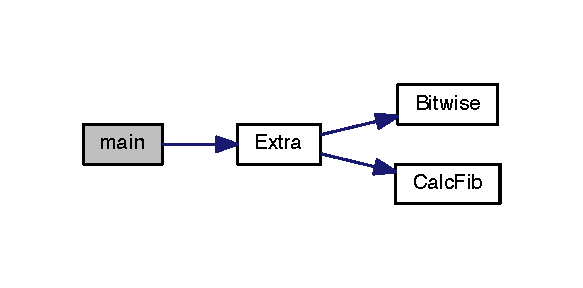
\includegraphics[width=280pt]{_expression_calc_8c_ae66f6b31b5ad750f1fe042a706a4e3d4_cgraph}
\end{center}
\end{figure}



\hypertarget{_r_e_a_d_m_e_8md}{\section{Developing\+Programming/\+Developing\+Computer\+Programming/\+R\+E\+A\+D\+M\+E.md File Reference}
\label{_r_e_a_d_m_e_8md}\index{Developing\+Programming/\+Developing\+Computer\+Programming/\+R\+E\+A\+D\+M\+E.\+md@{Developing\+Programming/\+Developing\+Computer\+Programming/\+R\+E\+A\+D\+M\+E.\+md}}
}

%--- End generated contents ---

% Index
\newpage
\phantomsection
\addcontentsline{toc}{chapter}{Index}
\printindex

\end{document}
